\documentclass{article} % Don't change this
\usepackage[a4paper, left=2.5cm, right=2cm, top=2cm, bottom=2cm]{geometry}
\usepackage[brazil]{babel}
\usepackage[utf8]{inputenc}

\newcommand{\trinum}[1]{%
	\triangle\hspace{-.57em}\raisebox{0.1em}{\scalebox{.5}{#1}}
}
\usepackage{lscape}
\usepackage{amsmath}
\usepackage{amsthm}
\usepackage{amsfonts}
\usepackage{amssymb}
\usepackage[usenames,dvipsnames]{xcolor}
\usepackage{graphicx}
\usepackage[siunitx]{circuitikz}
\usepackage{tikz}
\usepackage[colorinlistoftodos, color=orange!50]{todonotes}
\usepackage{hyperref}
%\usepackage[numbers, square]{natbib}
\usepackage{fancybox}
\usepackage{epsfig}
\usepackage{soul}
\usepackage[framemethod=tikz]{mdframed}
\usepackage{multirow}

\usepackage{gensymb}
\setcounter{MaxMatrixCols}{20}

\usepackage{paralist} %to enable {inparaenum}
\usepackage{natbib} %Natual bibliography
\usepackage{graphicx}
\usepackage{float} %To tables and figures
\usepackage{caption} %To describe figures
\usepackage{graphicx}
\usepackage{refstyle}
%\usepackage[latin1]{inputenc} %Type of decodification -Latinunderstandsportuguese acents
\usepackage{subcaption} % group of figures
%\usepackage{amsmath} %to enumerate an equantion according to section
\usepackage{booktabs} %to create tables
\usepackage{graphicx}
\usepackage{wrapfig}
\usepackage{amsmath}
\usepackage{multirow}
\usepackage{hyperref}%to show labels in red,blue and green colors
%\numberwithin{equation}{section} %to enumerate an equantion according to section
%\numberwithin{figure}{section} %to enumerate a figure according to section





\newcommand{\blah}{blah blah blah \dots}



\setlength{\marginparwidth}{3.4cm}

% NEW COUNTERS
\newcounter{points}
\setcounter{points}{100}
\newcounter{spelling}
\newcounter{usage}
\newcounter{units}
\newcounter{other}
\newcounter{source}
\newcounter{concept}
\newcounter{missing}
\newcounter{math}

% COMMANDS
%\newcommand{\raisa}[2]{\colorbox{Yellow}{#1} \todo{#2}}
\newcommand{\arbitrary}[2]{\todo{#1 #2} \addtocounter{points}{#2} \addtocounter{other}{#2}}
\newcommand{\english}{\todo{LANGUAGE (-1)} \addtocounter{points}{-1}
	\addtocounter{usage}{-1}}
\newcommand{\units}{\todo{UNITS (-1)} \addtocounter{points}{-1}
	\addtocounter{units}{-1}}
\newcommand{\spelling}{\todo{SPELLING and GRAMMAR (-1)} \addtocounter{points}{-1}
	\addtocounter{spelling}{-1}}
\newcommand{\source}{\todo{SOURCE(S) (-2)} \addtocounter{points}{-2}
	\addtocounter{source}{-2}}
\newcommand{\concept}{\todo{CONCEPT (-2)} \addtocounter{points}{-2}
	\addtocounter{concept}{-2}}
\newcommand{\missing}[2]{\todo{MISSING CONTENT (#1) #2} \addtocounter{points}{#1}
	\addtocounter{missing}{#1}}
\newcommand{\maths}{\todo{MATH (-1)} \addtocounter{points}{-1}
	\addtocounter{math}{-1}}

\newcommand{\summary}[1]{
	\begin{mdframed}[nobreak=true]
		\begin{minipage}{\textwidth}
			\vspace{0.5cm}
			\begin{center}
				\Large{Grade Summary} \hrule 
			\end{center} \vspace{0.5cm}
			General Comments: #1
			
			\vspace{0.5cm}
			Possible Points \dotfill 100 \\
			Points Lost (Spelling and Grammar) \dotfill \thespelling \\
			Points Lost (Language) \dotfill \theusage \\
			Points Lost (Units) \dotfill \theunits \\
			Points Lost (Math) \dotfill \themath \\
			Points Lost (Sources) \dotfill \thesource \\
			Points Lost (Concept) \dotfill \theconcept \\
			Points Lost (Missing Content) \dotfill \themissing \\
			Other \dotfill \theother \\[0.5cm]
			\begin{center}
				\large{\textbf{Grade:} \fbox{\thepoints}}
			\end{center}
		\end{minipage}
\end{mdframed}}


\renewcommand*{\thefootnote}{\fnsymbol{footnote}}


\title{
	\normalfont \normalsize 
	\textsc{Pontificia Universidade Católica do Rio de Janeiro, RJ, Brasil \\ 
		Departamento de Engenharia Civil e Ambiental, Geotecnia} \\
	[10pt] 
	\rule{\linewidth}{0.5pt} \\[6pt] 
	\huge LISTA Nº 1\\
	\rule{\linewidth}{2pt}  \\[10pt]
}
\author{Karen Ninanya}
\date{\normalsize (1812565)}

\begin{document}
	
	\maketitle
	\noindent
	Professor \dotfill Sergio Fontoura\\
	Disciplina \dotfill CIV 2534 - Mecânica das rochas aplicadas\\
	Data \dotfill 16 de Outobro, 2018 \\
	
	\newpage
	%\tableofcontents
	\newpage


\section*{Questão 1}

\vspace{10mm}
1. O objetivo deste exercício é trabalhar o conceito o conceito de distribução de tensões ao redor de uma abertura subterrânea.\\
2. Para tal será utilizada uma abertura circular num meio rochoso homogêneo isotrópico e linear elastica.\\
3. Considerar um estado de tensões \textit{in situ} definido por \(\sigma_v=40\) \(MPa\) e \(\sigma_h=30\) \(MPa\).\\
4. Considerar uma abertura de raio \(4,5\) \(m\).\\
5. Considerar uma rocha cuja resistência é definida por uma resistência à compressão simples de \(20\) \(MPa\) e um ângulo de atrito de \(35\degree\).\\
6. Determine a distribução de tensões utilizando as equações de Kirsch e estime a região de plastificação ao redor da abertura.




\newpage

\section*{Solução 1}

\vspace{10mm}


\underline{\large \textit{Método dos elementos finitos}}\\

\begin{itemize}
	\item Discretização
\end{itemize}

A discretizazção do medio poroso foe feita a partir de elementos de 3 nós (T3) , como pode ser observado na figura \ref{global}. A vista local do elemento é mostrado na figura \ref{local}.

\begin{figure}[H]
	\centering
	\caption{Vista global do problema com elementos de três nós (T3)}	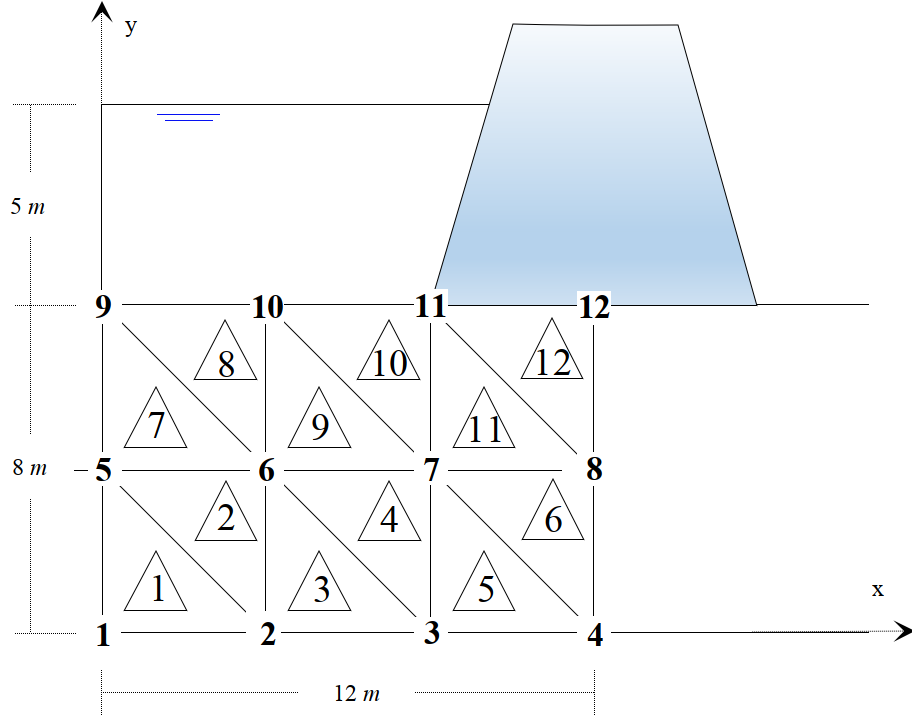
\includegraphics[width=0.65\linewidth]{elemento}	
	\label{global}	
\end{figure}
\begin{figure}[H]
	\centering
	\caption{Vista do elemento T3}	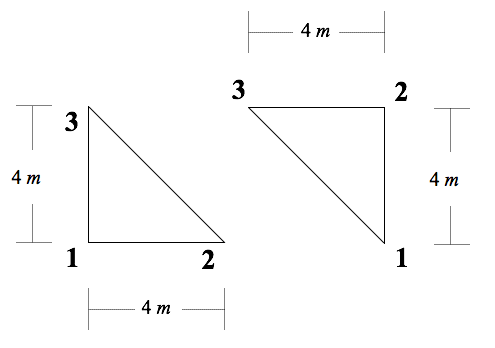
\includegraphics[width=0.45\linewidth]{local}	
	\label{local}	
\end{figure}
As coordenadas dos nós de acordo à figura \ref{global} são mostradas na seguinte tabela.
\begin{table}[H]
	\centering
	\begin{tabular}{@{}lcccccccccccc@{}}
		\toprule
		\multirow{2}{*}{Coordenadas} & \multicolumn{12}{c}{Nós} \\ \cmidrule(l){2-13} 
		& 1 & 2 & 3 & 4 & 5 & 6 & 7 & 8 & 9 & 10 & 11 & 12 \\ \midrule
		x (m) & 0 & 4 & 8 & 12 & 0 & 4 & 8 & 12 & 0 & 4 & 8 & 12 \\
		y (m) & 0 & 0 & 0 & 0 & 4 & 4 & 4 & 4 & 8 & 8 & 8 & 8 \\ \bottomrule
	\end{tabular}
\end{table}

\begin{itemize}
	\item Formulação variacional	
\end{itemize}


\begin{equation}
\Omega=\frac{1}{2}\int_{A}[q]^T[B]^T[R][B][q]dA-\int_{A}\bar{Q}[q]^T[N]^TdA-\int_{S_1}\bar{q}[q]^T[N]^TdS
\end{equation}

Ao derivar respecto de \([q]\), temos
\begin{equation}
\frac{\partial\Omega}{\partial [q]}=0=\int_{A}[B]^T[R][B][q]dA-\int_{A}\bar{Q}[N]^TdA-\int_{S_1}\bar{q}[N]^TdS
\end{equation}

\begin{equation}\label{geral}
\left[\int_{A}[B]^T[R][B]dA\right][q]=\left[\int_{A}\bar{Q}[N]^TdA+\int_{S_1}\bar{q}[N]^TdS\right]
\end{equation}

Agrupando.
\begin{equation}
[k][q]=[Q]
\end{equation}


\begin{itemize}
	\item Matriz elemental \([k]\)	
\end{itemize}

Da equação \ref{geral}, temos que a matriz elemental \([k]\) é a seguinte.
\begin{equation}
[k]=\int_{A}[B]^T[R][B]dA
\end{equation}
\begin{equation}\label{kelemento}
[k]=A[B]^T[R][B]
\end{equation}
onde o calculo das matrices \([R]\)  e \([B]\) é da seguinte manera.



\begin{equation}
[R]=\begin{bmatrix}
k_x&0\\0&k_y
\end{bmatrix}
\end{equation}

\begin{equation}
[B]=\frac{1}{2A}\begin{bmatrix}
y_{23}&y_{31}&y_{12}\\x_{32}&x_{13}&x_{21}
\end{bmatrix}
\end{equation}

sendo o calculo das áreas (\(A\)) da seguinte forma.

\begin{equation}
A=\frac{1}{2}\biggr|\color{white}\begin{bmatrix}\color{black}
1&\color{black}x_1&\color{black}y_1\\\color{black}1&\color{black}x_2&\color{black}y_2\\\color{black}1&\color{black}x_3&\color{black}y_3
\color{white}\end{bmatrix}\color{black}\biggr|
\end{equation}



Então, a matriz \([k]\) elemental ficaria:
\begin{equation}
[k]=\frac{1}{2\hspace{4pt}\biggr|\color{white}\begin{bmatrix}\color{black}
	1&\color{black}x_1&\color{black}y_1\\\color{black}1&\color{black}x_2&\color{black}y_2\\\color{black}1&\color{black}x_3&\color{black}y_3
	\color{white}\end{bmatrix}\color{black}\biggr|}\begin{bmatrix}
y_{23}&x_{32}\\y_{31}&x_{13}\\y_{12}&x_{21}
\end{bmatrix}\begin{bmatrix}
k_x&0\\0&k_y
\end{bmatrix}\begin{bmatrix}
y_{23}&y_{31}&y_{12}\\x_{32}&x_{13}&x_{21}
\end{bmatrix}
\end{equation}
onde \(k_x=k_y=k=1x10^{-6}m/s\)\\
Por tanto as matrices \([k]\) elementares do problema são os seguintes.


\begin{equation}
[k]^{1,3,5,7,9,11}=\frac{k}{2}\begin{bmatrix}
2&-1&-1\\-1&1&0\\-1&0&1
\end{bmatrix}
\end{equation}
\begin{equation}
[k]^{2,4,6,8,10,12}=\frac{k}{2}\begin{bmatrix}
1&-1&0\\-1&2&-1\\0&-1&1
\end{bmatrix}
\end{equation}


\begin{itemize}
	\item Vetor \([Q]\)	elementar
\end{itemize}


Logo, o vetor \([Q]\) de acordo a equação \ref{geral} e o seguinte.
\begin{equation*}
[{Q}]=\int_{A}\bar{Q}[N]^TdA+\int_{S_1}\bar{q}[N]^TdS
\end{equation*}

Sendo o valor do fluxo retirao ou injetado \(\bar{Q}=0\) os vetores \([Q]\) elementares são os mostrados a continuação.
\begin{equation*}
[{Q}]^{1}=[{Q}]^{2}=[{Q}]^{3}=[{Q}]^{4}=[{Q}]^{5}=[{Q}]^{6}=[{Q}]^{7}=[{Q}]^{8}=[{Q}]^{9}=[{Q}]^{10}=[{Q}]^{11}=[{Q}]^{12}=\begin{bmatrix}
0\\0\\0
\end{bmatrix}
\end{equation*}
\begin{itemize}
	\item Matriz de correspondencia Global-local
\end{itemize}



\begin{table}[H]
	\centering
	\begin{tabular}{@{}ccccccccccccc@{}}
		\toprule
		\multirow{2}{*}{Global} & \multicolumn{12}{c}{Local} \\ \cmidrule(l){2-13} 
		& $\trinum{1}$& $\trinum{2}$ & $\trinum{3}$ & $\trinum{4}$ &$\trinum{5}$ &$\trinum{6}$ &$\trinum{7}$ &$\trinum{8}$ &$\trinum{9}$ &$\trinum{10}$ &$\trinum{11}$ &$\trinum{12}$ \\ \midrule
		1 & 1 & - & - & - & - & - & - & -& - & - & - & -\\
		2 & 2 & 1 & 1& -& - & - & - & -& - & - & - & - \\
		3 & - & - & 2 & 1& 1 & - & - & -& - & - & - & - \\
		4 & - & -& - & - & 2 & 1& - & -& - & - & - & -\\
		5 & 3 & 3 & - & -& - & - & 1 & -& - & - & - & - \\
		6 & - & 2 & 3 & 3& - & - & 2 & 1& 1 & - & - & -\\
		7 & - & - & - & 2 & 3 & 3 & - & -& 2 & 1 & 1 & -\\
		8 & - & - & - & -& - & 2 & - & -& -& - & 2 & 1 \\
		9 & - & - & - & - & - & - & 3 & 3&- & - & - & -\\
		10 & - & - & - & - & -& - & - & 2& 3 & 3 & - & -\\
		11 & - & - & - & - & -& - & - & -&  & 2 & 3 & 3\\
		12 & - & - & - & - & - & - & - & -& - & - & - & 2\\ \bottomrule
	\end{tabular}
\end{table}



\begin{itemize}
	\item Montagem da matriz global
\end{itemize}


\begin{equation}
\frac{k}{2}\begin{bmatrix}
\color{red}2&\color{red}-1&\color{red}0&\color{red}0&\color{red}-1&\color{red}0&\color{red}0&\color{red}0&\color{red}0&\color{red}0&\color{red}0&\color{red}0\\
\color{red}-1&4&-1&\color{red}0&\color{red}0&-2&0&\color{red}0&\color{red}0&\color{red}0&\color{red}0&\color{red}0\\
\color{red}0&-1&4&\color{red}-1&\color{red}0&0&-2&\color{red}0&\color{red}0&\color{red}0&\color{red}0&\color{red}0\\
\color{red}0&\color{red}0&\color{red}-1&\color{red}2&\color{red}0&\color{red}0&\color{red}0&\color{red}-1&\color{red}0&\color{red}0&\color{red}0&\color{red}0\\
\color{red}-1&\color{red}0&\color{red}0&\color{red}0&\color{red}4&\color{red}-2&\color{red}0&\color{red}0&\color{red}-1&\color{red}0&\color{red}0&\color{red}0\\
\color{red}0&-2&0&\color{red}0&\color{red}-2&8&-2&\color{red}0&\color{red}0&\color{red}-2&\color{red}0&\color{red}0\\
\color{red}0&0&-2&\color{red}0&\color{red}0&-2&8&\color{red}-2&\color{red}0&\color{red}0&\color{red}-2&\color{red}0\\
\color{red}0&\color{red}0&\color{red}0&\color{red}-1&\color{red}0&\color{red}0&\color{red}-2&\color{red}4&\color{red}0&\color{red}0&\color{red}0&\color{red}-1\\
\color{red}0&\color{red}0&\color{red}0&\color{red}0&\color{red}-1&\color{red}0&\color{red}0&\color{red}0&\color{red}2&\color{red}-1&\color{red}0&\color{red}0\\
\color{red}0&\color{red}0&\color{red}0&\color{red}0&\color{red}0&\color{red}-2&\color{red}0&\color{red}0&\color{red}-1&\color{red}4&\color{red}-1&\color{red}0\\
\color{red}0&\color{red}0&\color{red}0&\color{red}0&\color{red}0&\color{red}0&\color{red}-2&\color{red}0&\color{red}0&\color{red}-1&\color{red}4&\color{red}-1\\
\color{red}0&\color{red}0&\color{red}0&\color{red}0&\color{red}0&\color{red}0&\color{red}0&\color{red}-1&\color{red}0&\color{red}0&\color{red}-1&\color{red}2
\end{bmatrix}\begin{bmatrix}
\color{red}h_1\\h_2\\h_3\\\color{red}h_4\\\color{red}h_5\\h_6\\h_7\\\color{red}h_8\\\color{red}h_9\\\color{red}h_{10}\\\color{red}h_{11}\\\color{red}h_{12}\\
\end{bmatrix}=\begin{bmatrix}
\color{red}0\\0\\0\\\color{red}0\\\color{red}0\\0\\0\\\color{red}0\\\color{red}0\\\color{red}0\\\color{red}0\\\color{red}0
\end{bmatrix}
\end{equation}
\begin{itemize}
	\item Introdução das condições de contorno
\end{itemize}

Sendo o valor das carga hidraulica \(h_1\), \(h_4\), \(h_5\), \(h_8\), \(h_9\), \(h_{10}\), \(h_{11}\) e \(h_{12}\) valores conhecidos o sistema linear fico da seguinte forma.


\begin{equation}
\begin{bmatrix}
4&-1&-2&0\\
-1&4&0&-2\\
-2&0&8&-2\\
0&-2&-2&8
\end{bmatrix}\begin{bmatrix}
h_2\\h_3\\h_6\\h_7
\end{bmatrix}=\begin{bmatrix}
h_1\\h_4\\2(h_5+h_{10})\\2(h_8+h_{11})
\end{bmatrix}=\begin{bmatrix}
13,00\\10,50\\52,00\\47,00
\end{bmatrix}
\end{equation}

Ao resolver o sistema linear no MatLab os valores das cargas hidraulicas \(h_2\), \(h_3\), \(h_6\) e \(h_7\) forem obtidos.
\begin{equation}
\begin{bmatrix}
h_1\\h_2\\h_3\\h_4\\h_5\\h_6\\h_7\\h_8\\h_9\\h_{10}\\h_{11}\\h_{12}
\end{bmatrix}=\begin{bmatrix}
13,00\\12,48\\11,72\\10,50\\13,00\\12,61\\11,96\\10,50\\13,00\\13,00\\13,00\\10,50
\end{bmatrix}m
\end{equation}

Na figura \ref{result} é mostrado as cargas hidraulicas nodais.
\begin{figure}[H]
	\centering
	\caption{Cargas hidraulicas em \(m\) e linhas equipotenciais de 11 \(m\) e 12 \(m\)}
	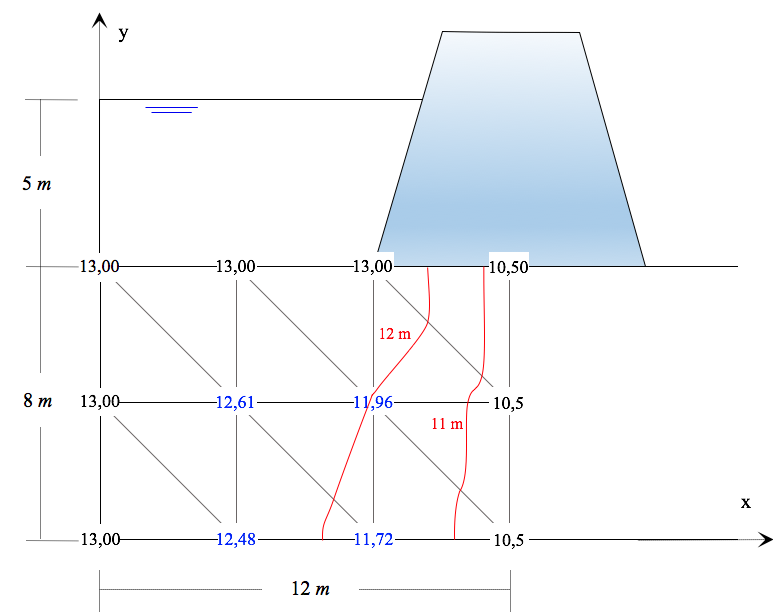
\includegraphics[width=0.75\linewidth]{result}	
	\label{result}	
\end{figure}


\begin{itemize}
	\item Variavel secundaria - Velocidade de fluxo
\end{itemize}


O calculo da velocidade de fluxo é determinada a partir da seguinte equiação.

\begin{equation}
[v]=-[R][g]
\end{equation}

sendo \([g]=[B][q]\), temos:

\begin{equation}
[v]=-[R][B][q]
\end{equation}

\begin{equation}\label{velocidade}
[v]=-\begin{bmatrix}
k_x&0\\
0&k_y
\end{bmatrix}\cdot\frac{1}{\hspace{4pt}\biggr|\color{white}\begin{bmatrix}\color{black}
	1&\color{black}x_1&\color{black}y_1\\\color{black}1&\color{black}x_2&\color{black}y_2\\\color{black}1&\color{black}x_3&\color{black}y_3
	\color{white}\end{bmatrix}\color{black}\biggr|}\begin{bmatrix}
y_{23}&y_{31}&y_{12}\\x_{32}&x_{13}&x_{21}
\end{bmatrix}\cdot \begin{bmatrix}
h_1\\
h_2\\
h_3
\end{bmatrix}
\end{equation}

 Reemplazando os correspondentes valores na equação \ref{velocidade} para cada elementos temos os correspondentes vetores de velocidade.
 
 
 \begin{equation}
 [v]^{1}=\begin{bmatrix}
1,30\\
0,00
 \end{bmatrix}\cdot 10^{-7}m/s
 \end{equation}
 
 \begin{equation}
[v]^{2}=\begin{bmatrix}
0,98\\
-0,33
\end{bmatrix}\cdot 10^{-7}m/s
\end{equation}

 \begin{equation}
[v]^{3}=\begin{bmatrix}
1,90\\
-0,33
\end{bmatrix}\cdot 10^{-7}m/s
\end{equation}

 \begin{equation}
[v]^{4}=\begin{bmatrix}
1,63\\
-0,60
\end{bmatrix}\cdot 10^{-7}m/s
\end{equation}

 \begin{equation}
[v]^{5}=\begin{bmatrix}
3,05\\
-0,60
\end{bmatrix}\cdot 10^{-7}m/s
\end{equation}

 \begin{equation}
[v]^{6}=\begin{bmatrix}
3,65\\
0,00
\end{bmatrix}\cdot 10^{-7}m/s
\end{equation}

 \begin{equation}
[v]^{7}=\begin{bmatrix}
0,98\\
0,00
\end{bmatrix}\cdot 10^{-7}m/s
\end{equation}
 \begin{equation}
[v]^{8}=\begin{bmatrix}
0,00\\
-0,98
\end{bmatrix}\cdot 10^{-7}m/s
\end{equation}
 \begin{equation}
[v]^{9}=\begin{bmatrix}
1,63\\
-0,98
\end{bmatrix}\cdot 10^{-7}m/s
\end{equation}

 \begin{equation}
[v]^{10}=\begin{bmatrix}
0,00\\
-2,60
\end{bmatrix}\cdot 10^{-7}m/s
\end{equation}

 \begin{equation}
[v]^{11}=\begin{bmatrix}
3,65\\
-2,60
\end{bmatrix}\cdot 10^{-7}m/s
\end{equation}

 \begin{equation}
[v]^{12}=\begin{bmatrix}
6,25\\
0,00
\end{bmatrix}\cdot 10^{-7}m/s
\end{equation}





\begin{figure}[H]
	\centering
	\caption{Velocidades nas direções x e y no meio poroso}
	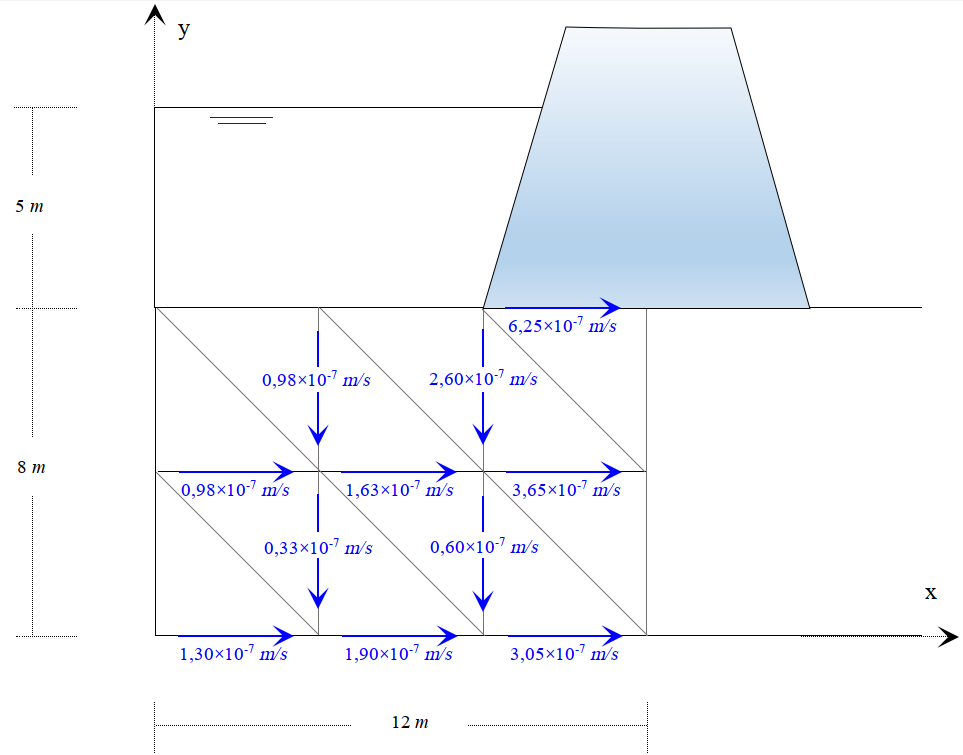
\includegraphics[width=1\linewidth]{velocidade}	
	\label{velocidadefinal}	
\end{figure}




%BIBLIOGRAPHY
%\bibliographystyle{apalike}
%\bibliography{bibliography}


\end{document}
